\documentclass{beamer}
\usepackage[utf8]{inputenc}

\usetheme{Madrid}
\usecolortheme{default}
\usepackage{amsmath,amssymb,amsfonts,amsthm}
\usepackage{txfonts}
\usepackage{tkz-euclide}
\usepackage{listings}
\usepackage{adjustbox}
\usepackage{array}
\usepackage{tabularx}
\usepackage{gvv}
\usepackage{lmodern}
\usepackage{circuitikz}
\usepackage{tikz}
\usepackage{graphicx}

\setbeamertemplate{page number in head/foot}[totalframenumber]

\usepackage{tcolorbox}
\tcbuselibrary{minted,breakable,xparse,skins}



\definecolor{bg}{gray}{0.95}
\DeclareTCBListing{mintedbox}{O{}m!O{}}{%
  breakable=true,
  listing engine=minted,
  listing only,
  minted language=#2,
  minted style=default,
  minted options={%
    linenos,
    gobble=0,
    breaklines=true,
    breakafter=,,
    fontsize=\small,
    numbersep=8pt,
    #1},
  boxsep=0pt,
  left skip=0pt,
  right skip=0pt,
  left=25pt,
  right=0pt,
  top=3pt,
  bottom=3pt,
  arc=5pt,
  leftrule=0pt,
  rightrule=0pt,
  bottomrule=2pt,
  toprule=2pt,
  colback=bg,
  colframe=orange!70,
  enhanced,
  overlay={%
    \begin{tcbclipinterior}
    \fill[orange!20!white] (frame.south west) rectangle ([xshift=20pt]frame.north west);
    \end{tcbclipinterior}},
  #3,
}
\lstset{
    language=C,
    basicstyle=\ttfamily\small,
    keywordstyle=\color{blue},
    stringstyle=\color{orange},
    commentstyle=\color{green!60!black},
    numbers=left,
    numberstyle=\tiny\color{gray},
    breaklines=true,
    showstringspaces=false,
}
%------------------------------------------------------------
%This block of code defines the information to appear in the
%Title page
\title %optional
{2.7.16}
\date{August 30, 2025}
%\subtitle{A short story}

\author % (optional)
{Aditya Appana - EE25BTECH11004}



\begin{document}


\frame{\titlepage}
\begin{frame}{Question}
Find $|\vec{a}\times \vec{b}|$ if $\vec{a} = (2\hat{i} +\hat{j} +3\hat{k})$ and  $ \vec{b}=(3\hat{i} + 5\hat{j} - 2\hat{k})$.
\end{frame}
\begin{frame}{allowframebreaks}
\frametitle{Given Information}

    \centering
    
    \label{tab:parameters}
    The vectors are
\begin{align} 
\vec{a} = \myvec{2\\1\\3}\\
\vec{b} = \myvec{3\\5\\-2}
\end{align}
\end{frame}

\begin{frame}{Formula}

To calculate the cross-product of the two vectors \vec{a} and \vec{b}, we use the following determinant:
\begin{center}
\myvec{|\vec{A_{23}} \vec{B_{23}}| \\ |\vec{A_{31}}   \vec{B_{31}}| \\ |\vec{A_{12}} \vec{B_{12}}| }
\end{center}


Where \vec{X_{ij}} = \myvec{$x_i$ \\ $x_j$}.

\end{frame}


\begin{frame}[fragile]
    \frametitle{Solution}

Expanding the determinants, we get: 
\begin{align}
\myvec{ ((-2) - 15) \\ ((-4) - 9) \\ (10-3)}  \\
= \myvec{-17\\13\\7} 
\end{align}

We need to find the norm of this vector, which is done by:
\begin{align}
\sqrt{17^2+13^2+7^2} \\
=22.516660498395403
\end{align}


\end{frame}


\begin{frame}[fragile]
    \frametitle{Python Code}
    \begin{lstlisting}
import numpy as np
import math
import matplotlib.pyplot as plt
import numpy.linalg as LA

vecA = np.array([2,1,3])
vecB = np.array([3,5,-2])

crossprod = np.cross(vecA,vecB)
print(crossprod)

mod = np.linalg.norm(crossprod)
print(mod)

\end{lstlisting}
\end{frame}

\begin{frame}[fragile]
    \frametitle{Python Code}

    \begin{lstlisting}
fig = plt.figure(figsize=(8, 8))
ax = fig.add_subplot(111, projection='3d')
origin = np.array([0, 0, 0])

ax.quiver(*origin, *vecA, color='r', label='Vector (3, 5, -2)')
ax.quiver(*origin, *vecB, color='b', label='Vector (2, 1, 3)')

max_val = np.max(np.abs(np.concatenate((vecA, vecB))))
ax.set_xlim([-max_val, max_val])
ax.set_ylim([-max_val, max_val])
ax.set_zlim([-max_val, max_val])
ax.set_xlabel('X-axis')
ax.set_ylabel('Y-axis')
ax.set_zlabel('Z-axis')
ax.set_title('3D Vectors')

ax.legend()
ax.grid(True)
plt.show()
    \end{lstlisting}
\end{frame}


\begin{frame}{Plot}
\begin{figure}
    \centering
    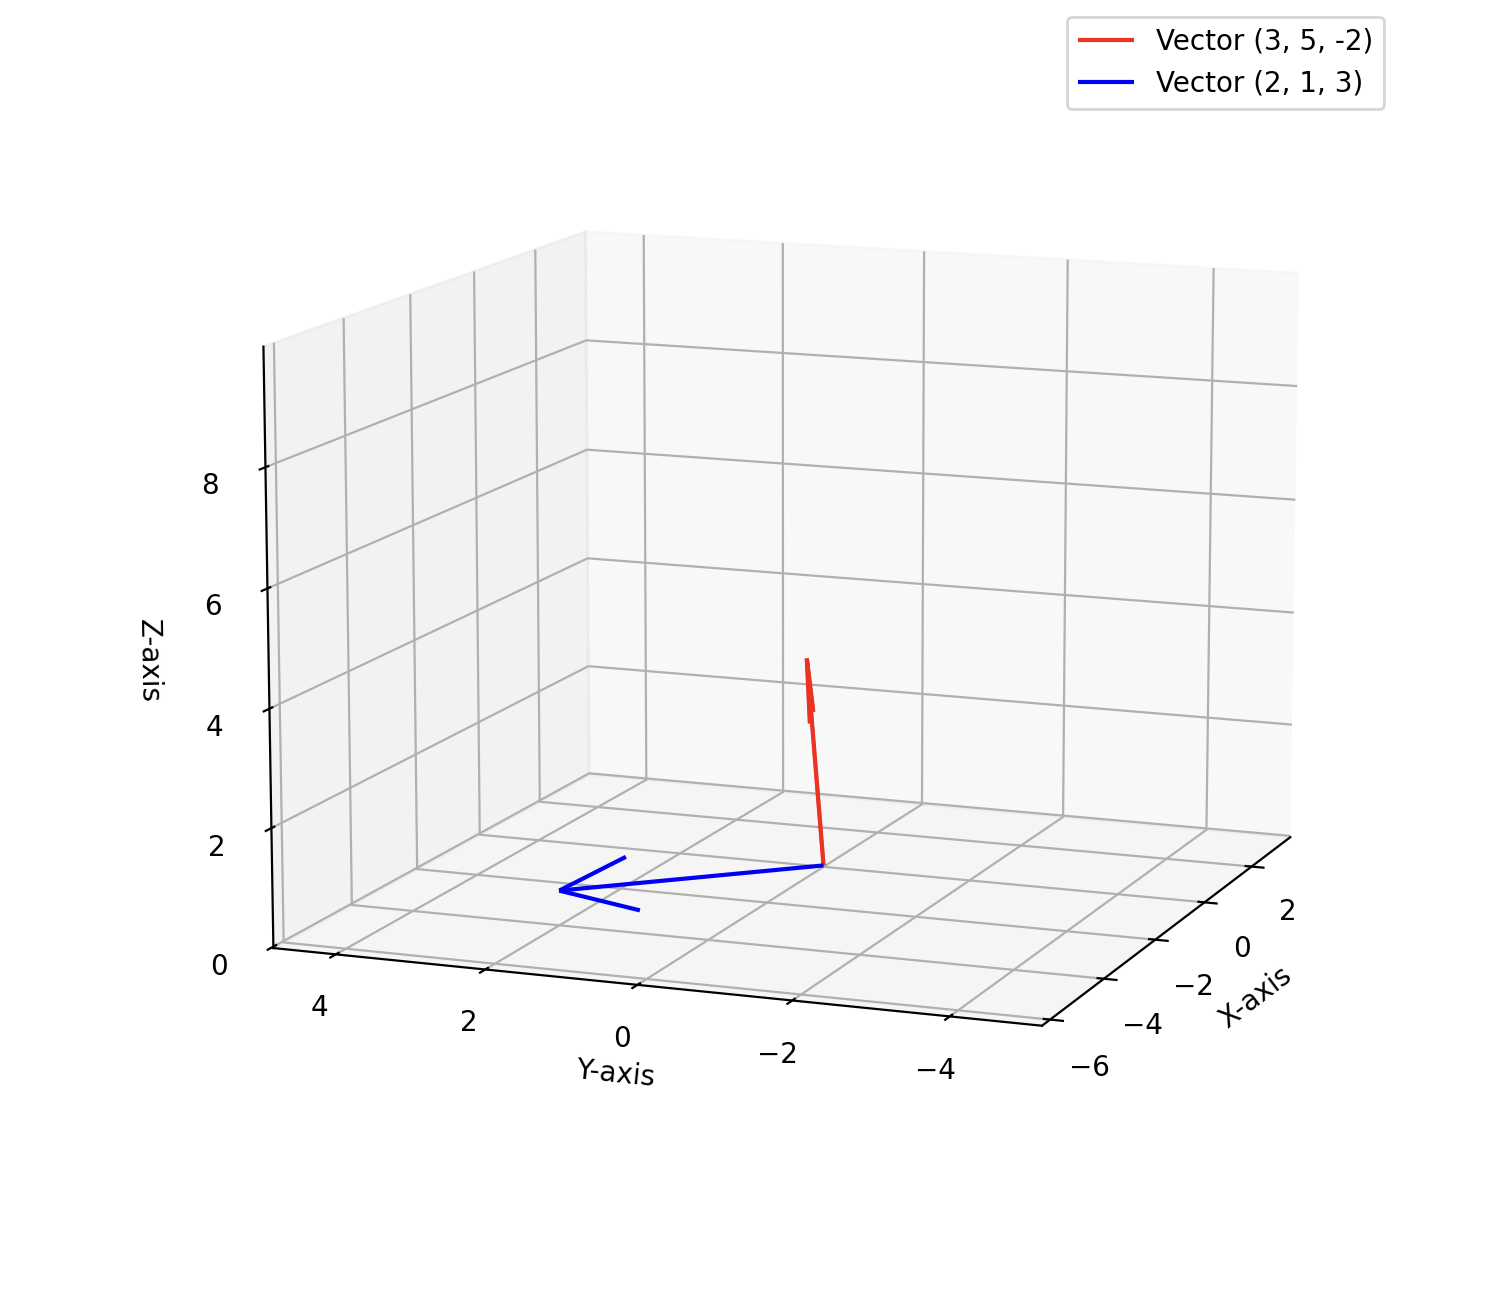
\includegraphics[width=0.8\columnwidth]{Figs/Figure_4.png}
    \caption{Plot}
    \label{fig:placeholder}
\end{figure}
\end{frame}


\begin{frame}[fragile]
\frametitle{C Code}
\begin{lstlisting}
#include<stdio.h>
#include<math.h>

int crossprod(float a0, float a1, float a2, float b0, float b1, float b2){

float modA = sqrt(pow(a0,2)+pow(a1,2)+pow(a2,2));
float modB = sqrt(pow(b0,2)+pow(b1,2)+pow(b2,2));

float dotprod = a0*b0 + a1*b1 + a2*b2;

float mod = sqrt(pow(modA,2)*pow(modB,2) - pow(dotprod,2));

return mod;
}
\end{lstlisting}

\end{frame}

\begin{frame}[fragile]
\frametitle{Python and C Code}

\begin{lstlisting}
import numpy as np
import ctypes
import matplotlib.pyplot as plt
c_lib=ctypes.CDLL('./4c.so')

c_lib.crossprod.argtypes = [ctypes.c_float, ctypes.c_float,ctypes.c_float, ctypes.c_float, ctypes.c_float, ctypes.c_float]
c_lib.crossprod.restype = ctypes.c_float
vecA = np.array([2,1,3])
vecB = np.array([3,5,-2])

mod = c_lib.crossprod(
    ctypes.c_float(vecA[0]),
    ctypes.c_float(vecA[1]), 
    ctypes.c_float(vecA[2]),
    ctypes.c_float(vecB[0]), 
    ctypes.c_float(vecB[1]),
    ctypes.c_float(vecB[2]))
\end{lstlisting}

\end{frame}

\begin{frame}[fragile]
\frametitle{Python and C Code}
\begin{lstlisting}
print(mod)
vecA = np.array([2,1,3]).reshape(-1,1)
vecB = np.array([3,5,-2]).reshape(-1,1)

fig = plt.figure(figsize=(8, 8))
ax = fig.add_subplot(111, projection='3d')

origin = np.array([0, 0, 0])

ax.quiver(*origin, *vecA, color='r', label='Vector (3, 5, -2)')
ax.quiver(*origin, *vecB, color='b', label='Vector (2, 1, 3)')

max_val = np.max(np.abs(np.concatenate((vecA, vecB))))
\end{lstlisting}

\end{frame}

\begin{frame}[fragile]
\frametitle{Python and C Code}

\begin{lstlisting}
ax.set_xlim([-max_val, max_val])
ax.set_ylim([-max_val, max_val])
ax.set_zlim([-max_val, max_val])

ax.set_xlabel('X-axis')
ax.set_ylabel('Y-axis')
ax.set_zlabel('Z-axis')
ax.set_title('Two 3D Vectors')

ax.legend()
ax.grid(True)
plt.show()
\end{lstlisting}

\end{frame}


\begin{frame}{Plot}
\begin{figure}
    \centering
    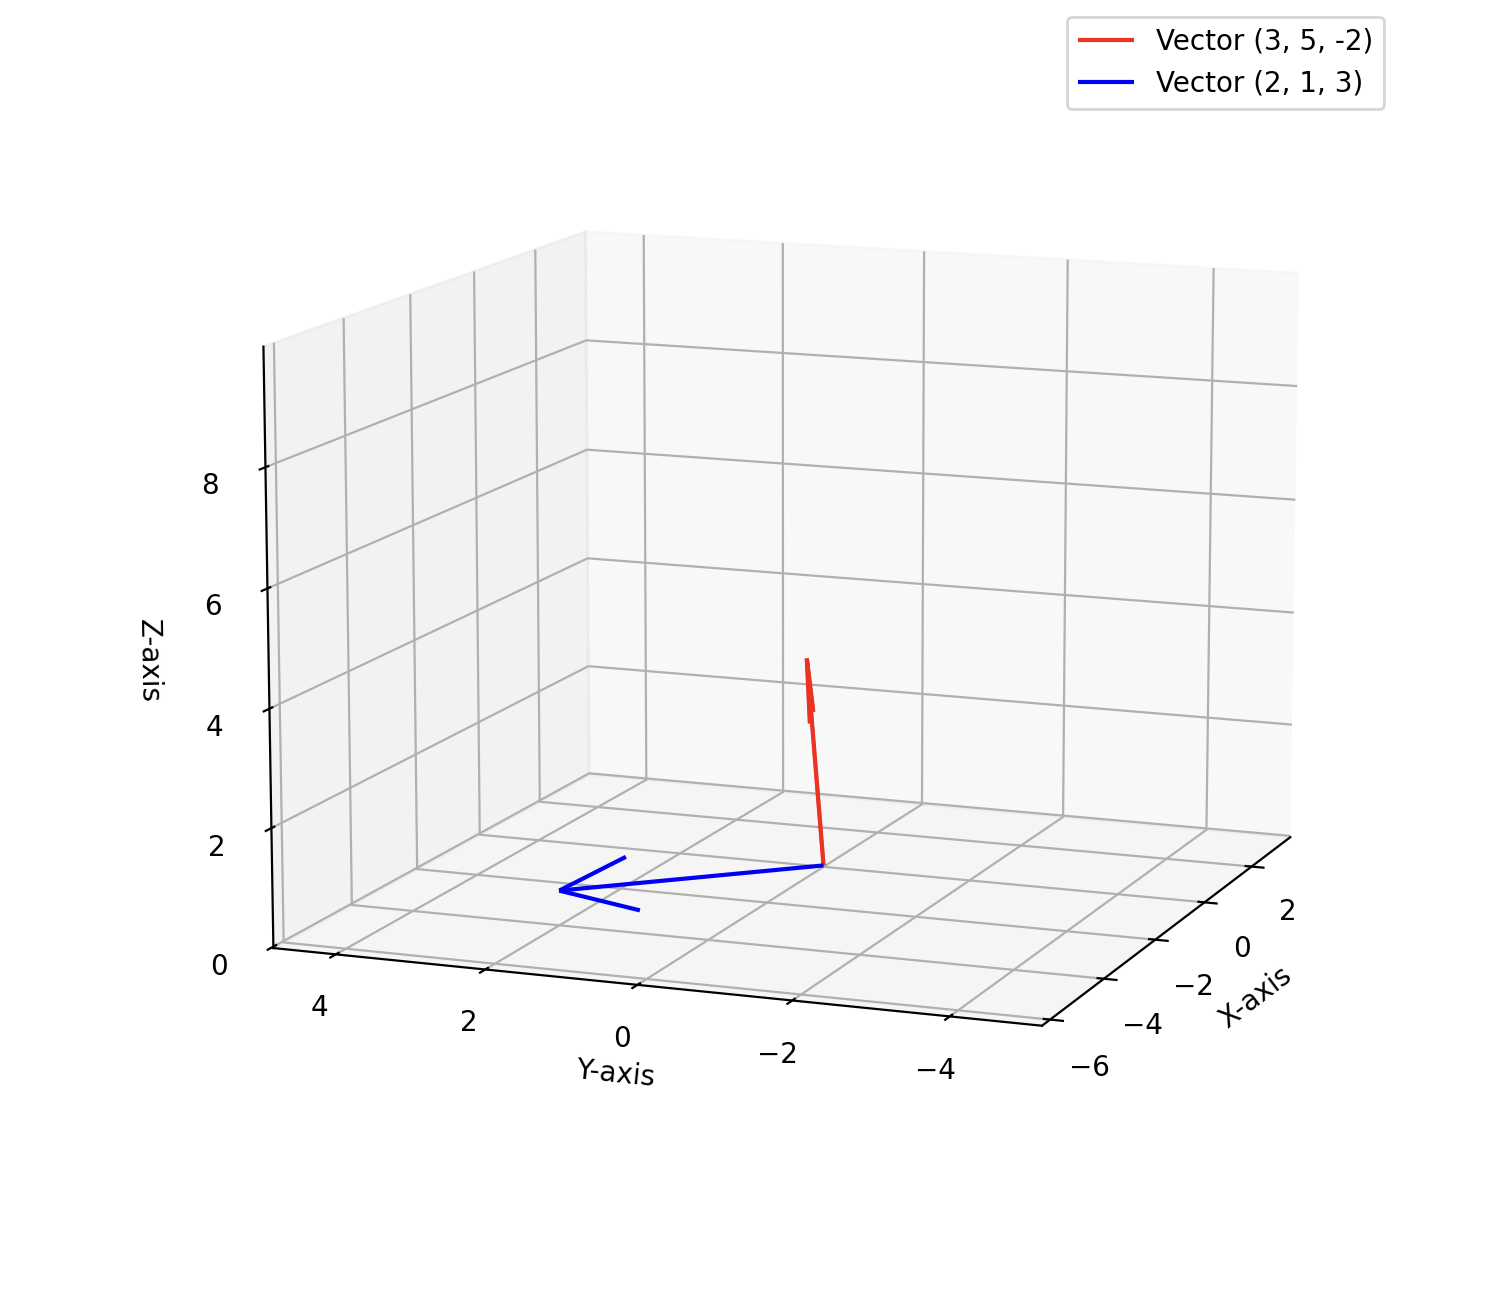
\includegraphics[width=0.8\columnwidth]{Figs/Figure_4.png}
    \caption{Plot}
    \label{fig:placeholder}
\end{figure}
\end{frame}

\end{document}